\chapter{Projeto Conceitual do Produto}

\section{Características gerais}

\textcolor{red}{Descrever produto de forma geral. Apresentar itens teóricos sobre o projeto a serem aprofundados ou detalhados oportunamente.}

\textcolor{red}{Apresentar e explicar a Estrutura Analítica do Projeto (EAP), tomando cuidado com a legibilidade da imagem. Se necessário, coloque a EAP dentro do comando ``\textsf{\textbackslash begin\{landscape\} \textbackslash end\{landscape\}}'' para que ela seja apresentada em uma página deitada.}

\section{Estrutura}

\textcolor{red}{Apresentar desenho em CAD, indicar dimensões por lado/aresta/cota, indicar materiais utilizados e explicar o desenho e as decisões de projeto.}

\section{Descrição de \textit{hardware}}

\textcolor{red}{A descrição de \textit{hardware} no documento deve permitir que outras pessoas repliquem o produto proposto neste documento. Para isso, deve-se explicar de forma textual os principais sub-sistemas e as escolhas de projeto, além de indicar:}

\begin{itemize}
    \item \textcolor{red}{ O diagrama de blocos \cite{blockdiagram}, que oferece uma visão geral do hardware, com as principais partes do sistema e as ligações entre elas.}
    %\item A lista de materiais \cite{bom}, que facilita a montagem do sistema, indicando tudo que deve ser adquirido. Aproveitem a lista de materiais para apresentarem o orçamento dos mesmos.
    \item \textcolor{red}{ O esquemático \cite{esquematico}, que mostra as conexões elétricas entre os componentes. Deve-se indicar os componentes por nomes e símbolos, e as conexões entre eles, incluindo a pinagem dos componentes. Se o esquemático ficar muito grande, pode-se separa-lo em vários esquemáticos. A ligação em \textit{protoboard} não é considerada um esquemático adequado.}
\end{itemize}

\textcolor{red}{A Fig. \ref{fig:diagrama_blocos_e_esquematico} apresenta o diagrama de blocos e o esquemático de um circuito conversor de corrente alternada para corrente direta, a título de exemplo. Repare que o diagrama de blocos indica os subsistemas do circuito completo apresentado no esquemático.
% Comecem com o diagrama de blocos, que é mais genérico, e depois indiquem os detalhes com a lista de materiais e os esquemáticos.
}

\begin{figure}
    \centering
    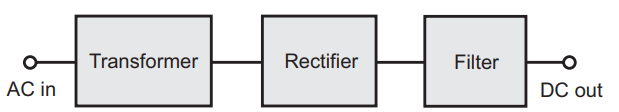
\includegraphics[width=0.5\linewidth]{figuras/Exemplo-diagrama-de-blocos.png}
    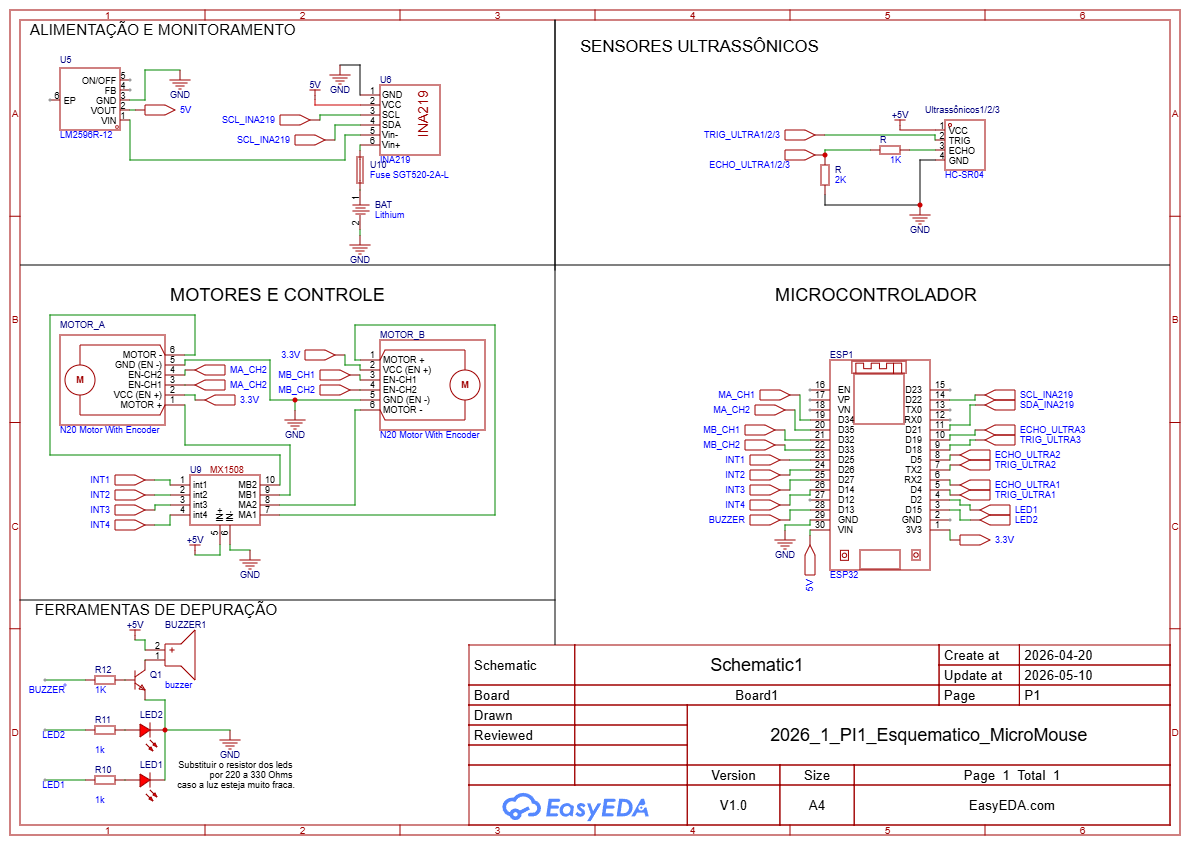
\includegraphics[width=0.5\linewidth]{figuras/Esquematico.png}
    \caption{\textcolor{red}{Diagrama de blocos e esquemático de um circuito conversor de corrente alternada para corrente direta. Extraído de \cite{block_n_schematic}.}}
    \label{fig:diagrama_blocos_e_esquematico}
\end{figure}

\section{Análise de consumo energético}

\textcolor{red}{Com relação ao consumo energético do produto desenvolvido, será necessário apresentar cálculos de consumo dos diversos componentes utilizados e explicar as decisões de projeto para atender a estas demandas.}


\section{Análise de consumo energético}

Abaixo, apresenta-se o detalhamento do consumo energético do sistema, considerando os componentes selecionados e o regime de operação previsto para o produto.

\begin{itemize}
    \item \textbf{Identificação dos Subsistemas Elétricos:} 
    O sistema é alimentado por uma bateria de 12V, cuja tensão é reduzida para o funcionamento dos demais componentes. O tempo estimado de operação contínua é de 7200 segundos (2 horas):
    \begin{itemize}
        \item \textbf{Microcontrolador (ESP32 DevKit):} 5V, 150mA, 7200s.
        \item \textbf{Atuadores (2x Motores N20):} 5V (via regulador), 240mA total, 7200s.
        \item \textbf{Sensores (Ultrassônicos):} 5V, 45mA, 7200s.
        \item \textbf{Indicadores (Buzzer e LEDs):} 5V, 40mA, 7200s.
        \item \textbf{Monitoramento (Sensor INA219):} 5V, 1mA, 7200s.
    \end{itemize}

    \item \textbf{Cálculo da Energia Consumida por Componente:} 
    Os cálculos foram realizados utilizando a fórmula $E = V \cdot I \cdot t$:
    \begin{itemize}
        \item $E_{ESP32} = 5V \times 0,150A \times 7200s = 5.400$ J
        \item $E_{Motores} = 5V \times 0,240A \times 7200s = 8.640$ J
        \item $E_{Sensores} = 5V \times 0,045A \times 7200s = 1.620$ J
        \item $E_{Indicadores} = 5V \times 0,040A \times 7200s = 1.440$ J
        \item $E_{INA219} = 5V \times 0,001A \times 7200s = 36$ J
    \end{itemize}

    \item \textbf{Estimativa do Consumo Total de Energia:} 
    A energia total consumida estimada para o ciclo é de \textbf{17.136 Joules}. Considerando o consumo médio de 476 mA, a demanda prevista para 2 horas de uso é de aproximadamente \textbf{952 mAh}.

    \item \textbf{Escolha da Fonte de Alimentação:} 
    O consumo total equivale a 4,76 Wh. A bateria selecionada (Li-ion 3x18650, 12V, 2000 mAh) fornece 24 Wh, garantindo uma margem de segurança superior a 50\%, o que é ideal para compensar perdas térmicas e picos de corrente.

    \item \textbf{Planejamento do Circuito de Alimentação:} 
    Utiliza-se o regulador de tensão \textbf{LM2596 (Step-Down)} para converter os 12V da bateria em 5V estáveis. O circuito conta com o sensor \textbf{INA219} para monitoramento de corrente e tensão, servindo como proteção contra sobrecargas.

    \item \textbf{Monitoramento via \textit{software}:} 
    O ESP32 realiza a leitura do sensor INA219 via código, permitindo acompanhar o consumo em tempo real e registrar o tempo de operação para evitar a descarga profunda da bateria.

    \item \textbf{Validação com Testes Reais:} 
    A validação compara a autonomia teórica com a real. Diferenças encontradas são atribuídas à eficiência do LM2596 (80-90\%) e dissipação por Efeito Joule nos condutores.
\end{itemize}

\section{Descrição de \textit{software}}

\textcolor{red}{Itens fundamentais:}

\begin{itemize}
    \item \textcolor{red}{ \textbf{Diagrama Atividades UML:}  descrever e explicar o fluxo do comportamento funcional do produto proposto, evidenciando, de forma clara e estruturada, como as atividades são executadas, em que ordem e sob quais condições. Esse diagrama permite compreender o funcionamento dinâmico do sistema, destacando:}

    \begin{itemize}
        \item \textcolor{red}{ os principais atores (usuários ou sistemas externos) envolvidos no processo;
        \item as atividades de negócio realizadas por cada ator ou pelo próprio sistema;
        \item os insumos (entradas) necessários para a execução das atividades;
        \item os resultados (saídas) gerados ao longo do fluxo;
        \item os pontos de decisão, paralelismo e sincronização das atividades;
        \item Entre as notações mais relevantes, destacam-se o estado iniciail e final, atividades, nós de decisão e junção, barras de bifurcação, Raias (\textit{swimlanes}) e Fluxos de controle. }
        \end{itemize}

    \item \textcolor{red}{\textbf{\textit{Backlog} do Produto}}
    \begin{itemize}
        \item \textcolor{red}{ Descrever os   requisitos funcionais (RF) com a técnica de documentação e especificação de história de usuário (HU);}
        \item \textcolor{red}{ Descrever os requisitos não-funcionais (RNF) de forma objetiva; Mais facilmente, mais rapidamente, mais responsivo, de fácil uso, são descrições subjetivas não-válidas. Um exemplo de requisito não-funcional de desempenho: ``a página deve carregar em até 5s quando em conexão 4G''. }
        \item \textcolor{red}{ Ao descrever os requisitos (RF e RNF), usar a  classificação MoSCoW (\textit{Must have}, \textit{Should have} e \textit{Could have}),  para auxiliar a priorização dos itens do backlog.}
        \item \textcolor{red}{ Protótipos de interfafe gráfica do \textit{software} em alta fidelidade.}
        \begin{itemize}
            \item \textcolor{red}{\textbf{ Todas HUs devem conter sua descrição (Eu-Como-Para), critérios de aceitação e protótipos de interface, documentadas no github. }}
            \end{itemize} 

        \end{itemize}

    \item \textcolor{red}{ \textbf{Descrição da arquitetura da solução de \textit{software} proposta:}}
    \begin{itemize}
    
        \item \textcolor{red}{ Esta subseção deve contemplar o documento de arquitetura do sistema e deve ser estruturado segundo as visões (4+1) previstas no processo unificado (UP): lógica, de processos;  implementação, implantação e dados (substuirá a visão de casos de uso).}
        
        \item \textcolor{red}{ Propósito do \textit{software} (qual o seu papel no sistema);}
        \item \textcolor{red}{ Padrão adotado: MVC, MVP, Microsserviços, Monolítico, etc (Justificar);}
        \item \textcolor{red}{ Linguagens de programação: Java, Python, C\#, JavaScript, etc.}
        \item \textcolor{red}{ \textit{Frameworks} e bibliotecas: Spring Boot, .NET Core, React, Angular, Django, etc.}
            \item \textcolor{red}{ Banco de dados: Relacional (PostgreSQL, MySQL, etc) X NãoSQL (MongoDB,etc). }
        \item \textcolor{red}{Persistência de dados: Modelo Entidade‑Relacionamento (MER) e seu respectivo Diagrama Entidade‑Relacionamento (DER), aplicáveis quando a solução utiliza banco de dados relacional; alternativamente, diagrama de estrutura de documentos, empregado nos casos em que a arquitetura adota banco de dados não relacional.}
         \end{itemize}     
    
    \item \textcolor{red}{\textbf{ Roteiro de testes funcionais:} }
    \begin{itemize}
        \item \textcolor{red}{Código do caso de teste;}
        \item \textcolor{red}{Nome do caso de teste;}
        \item \textcolor{red}{ Objetivo do caso de teste;}
        \item \textcolor{red}{ Pré-condições do sistema para o teste ser realizado, quando se aplicar;}
        \item \textcolor{red}{ Descrição dos procedimentos a serem executados para o teste;}
        \item \textcolor{red}{ Resultado esperado para o teste ser aprovado (pós-condição após realizado o teste);}
    \end{itemize}
\end{itemize}
